% $Id: template.tex 11 2007-04-03 22:25:53Z jpeltier $
\documentclass{vgtc}                          % final (conference style)

\ifpdf%                                % if we use pdflatex
  \pdfoutput=1\relax                   % create PDFs from pdfLaTeX
  \pdfcompresslevel=9                  % PDF Compression
  \pdfoptionpdfminorversion=7          % create PDF 1.7
  \ExecuteOptions{pdftex}
  \usepackage{graphicx}                % allow us to embed graphics files
  \DeclareGraphicsExtensions{.pdf,.png,.jpg,.jpeg} % for pdflatex we expect .pdf, .png, or .jpg files
\else%                                 % else we use pure latex
  \ExecuteOptions{dvips}
  \usepackage{graphicx}                % allow us to embed graphics files
  \DeclareGraphicsExtensions{.eps}     % for pure latex we expect eps files
\fi%

%% it is recomended to use ``\autoref{sec:bla}'' instead of ``Fig.~\ref{sec:bla}''
\graphicspath{{figures/}{pictures/}{images/}{./}} % where to search for the images

\usepackage{microtype}                 % use micro-typography (slightly more compact, better to read)
\PassOptionsToPackage{warn}{textcomp}  % to address font issues with \textrightarrow
\usepackage{textcomp}                  % use better special symbols
\usepackage{mathptmx}                  % use matching math font
\usepackage{times}                     % we use Times as the main font
\renewcommand*\ttdefault{txtt}         % a nicer typewriter font
\usepackage{tabu}                      % only used for the table example
\usepackage{booktabs}                  % only used for the table 
\usepackage{url}
\usepackage{tabularray}
\usepackage[backend=biber]{biblatex}
\usepackage{cleveref}
\addbibresource{template.bib}

\onlineid{0}
\vgtccategory{Research}

\title{The State-of-Art Platforms and Tools for Immersive Analytical
Applications Development}

\author{Walid Chtioui\thanks{e-mail: walid.chtioui@ensi-uma.tn}\\ %
        \scriptsize University of Passau %
\and Achraf Hebheb\thanks{e-mail: habhabachref@gmail.com}\\ %
     \scriptsize University of Passau}

%% A teaser figure can be included as follows, but is not recommended since
%% the space is now taken up by a full width abstract.
%\teaser{
%  \includegraphics[width=1.5in]{sample.eps}
%  \caption{Lookit! Lookit!}
%}

\abstract{This paper presents an overview of the latest state-of-the-art
platforms and toolkits which can be used to develop immersive analytics (IA)
experiences. Initially, a short overview of Unity3D and Unreal Engine with a
comparison of supported eXtended Reality (XR) features and third party tools
is provided. After that, we present an overview associated with a critique of
what we believe are the major XR development toolkits. For each toolkit we
discuss the set of what we think are important features they provide or lack
such as the support for collaboration, interactions, real-time data and large
datasets. We then present a comparison study between these toolkits with a
particular focus on performance, supported devices, accessibility and
ease-of-use. A set of state-of-the-art tools and techniques, which can be used
to extend aforementioned toolkits, covering collaboration, interaction and
navigation topics are then provided. We've come to the conclusion that,
although IA toolkits have come out of their infancy, we are still yet to see an
IA toolkit that provides a unified workflow allowing for versatile
visualizations, collaboration support, acceptable performance scalability,
real-time data support and support for a plethora of XR and non-XR devices
which has the potential to replicate the wide success of conventional
visualization frameworks such as D3.js.
} % end of abstract

%%%%%%%%%%%%%%%%%%%%%%%%%%%%%%%%%%%%%%%%%%%%%%%%%%%%%%%%%%%%%%%%%%%%%%%%%%%%%%%
%%%%%%%%%%%%%%%%%%%%%%%%%%%%%% START OF THE PAPER %%%%%%%%%%%%%%%%%%%%%%%%%%%%%
%%%%%%%%%%%%%%%%%%%%%%%%%%%%%%%%%%%%%%%%%%%%%%%%%%%%%%%%%%%%%%%%%%%%%%%%%%%%%%%

\begin{document}
\firstsection{Introduction}
\maketitle



\section{Platforms}
\subsection{Unity}
Unity has a wide adoption in the world of XR thanks to its unified workflow
and support for various XR platforms - build once, run
everywhere -. Unity supports an extensive set of XR vendor-specific software
development kits (hereafter SDK) including: Apple's ARKit, Google's ARCore,
Microsoft's HoloLens and OpenXR. Following the announcement of Apple's
mixed reality (MR) headset Vision Pro in Apple's Worldwide Developers
Conference (WWDC) 2023, Unity was announced to provide native support for
Vision's Pro operating system VisionOS \cite{web:vision_pro_unity}.
Unity also provides a set of XR packages that are built on top of these vendor
plugins to add application-level development tools \cite{unity:xr_packages}.
For instance, AR Foundation is an industry-standard framework that provides
support for various AR features such as: object tracking and plane detection.
Unity also provides XR Interaction Toolkit package which is a high-level,
component-based interaction system. The package also includes XR Device
Simulator which is a simulator that allows user input from conventional input
devices (a keyboard, a mouse or a controller) to drive XR headset and
controllers in the Unity scene view. This may be useful for debugging on a
wide range of XR devices without having to actually try them. Unity also
benefits from open-source external XR packages such as the Mixed Reality
Toolkit for Unity (MRTK)
\footnote{https://github.com/MixedRealityToolkit/MixedRealityToolkit-Unity}
which is designed to further accelerate cross-platform MR development in Unity.
\subsection{Unreal Engine}
\subsection{Comparison}
Figure \ref{table:1} provides a comparison between the previously discussed
platforms in terms of support for vendor-specific SDKs and a set of features.

\begin{table}[ht!]
	\centering

	\begin{tabular}{l c c}
		\toprule
		                              & \multicolumn{2}{c}{\textbf{Platform}}                     \\
		\cmidrule(l){2-3}
		\textbf{SDKs}                 & Unity 2022 LTS                        & Unreal Engine 5.3 \\
		\midrule
		ARCore                        & X                                     & X                 \\
		ARKit                         & X                                     & X                 \\
		Magic Leap                    & X                                     & X                 \\
		Microsof HoloLens             & X                                     & X                 \\
		OpenXR                        & X                                     & X                 \\
		Oculus                        & X                                     & X                 \\
		WebXR                         & X                                     &                   \\
		VisionOS                      & X                                     &                   \\
		\midrule
		\textbf{AR-Specific Features} &                                       &                   \\
		\midrule
		Plane Detection               & X                                     & X                 \\
		Object Occlusion              & X                                     & X                 \\
		Environment Probes            & X                                     & X                 \\
		Face Tracking                 & X                                     & *(ARKit only)     \\
		Object Tracking               & X                                     & X                 \\
		Body Tracking                 & X                                     & ? (not mentioned) \\
		Camera Intrinsics             & X                                     & X                 \\
		Meshing                       & X                                     & ? (not mentioned) \\
		\midrule
		\textbf{XR Features}          &                                       &                   \\
		\midrule
		High-level XR Interactions    & X                                     & ? (not mentioned) \\
		XR Input Simulation           & X                                     & ? (not mentioned) \\
		\midrule
		Vuforia Support               & X                                     &                   \\
		\bottomrule
	\end{tabular}


	\medskip

	\caption{Per-platform supported SDKs, AR features and 3rd party tools.}
	\label{table:1}
\end{table}

\section{Toolkits and Frameworks}

The term toolkit refers to development environments that are tailor-made for
IA experience development purposes. They provide, among other things,
high-level tools for authoring visualizations, built-in interactions and
support for multiple major XR devices.

\subsection{DXR Toolkit}

Sicat et al. proposed DXR \cite{dxr_toolkit}; an IA toolkit built on top of Unity
that allows fast prototyping and iteration for non-experienced users; i.e.
users with no or little programming knowledge in XR and Unity.
Alongside the data input, DXR takes a specification file written in JavaScript
Object Notation (hereafter JSON) from which visualisations are created.
The specification file is described in Vega-Lite declarative grammar \cite{vega_lite}
(only what should be achieved has to be provided, not how) making it suitable
for users with no programming experience to rapidly realise immersive
visualisations. This configuration file can be edited in a separate text editor or through
the use of a GUI with pre-configured set of parameters. DXR also provides
built-in specification templates for common visualisations such as: Scatter
plots and bar charts. This further extends the scope of users to include
those without any technical experience. Although the authors claim that DXR
provides suitable flexibility, the scope of that flexibility seems to be
limited, among other things, to providing custom graphical markers, custom
visualization channels - a visualization channel is a visualisation parameter affected by some
data dimension(s), such as object color affected by temperature data dimension in some dataset -
and other visualisation-type specific properties. That limits users to a
templated and common set of visualisations such as scatter plots, bar charts
and radial bars. There is also no mention of real-time data support thus
limiting the use case of DXR to offline data only.

\smallskip

\noindent As the authors have explicitly mentioned, DXR is meant for
prototyping and exploring designs, it is not designed to handle visualisations
of large datasets. On HoloLens, for datasets with more than approximately
a thousand item, suboptimal - less that 60 frames per second (hereafter FPS) -
performance has been observed. Nonetheless, the authors argue that DXR can still
be useful for quickly and cheaply prototyping large dataset designs before
moving to specialized, optimized and detailed implementations.

\subsection{IATK Toolkit}
Maxime et al. introduced IATK \cite{iatk_toolkit}; an open-source
\footnote{https://github.com/MaximeCordeil/IATK} software
package for Unity that provides both a high-level Unity-editor-integrated GUI
for simple authoring and a low-level C-sharp and JavaScript API for
fine-grained authoring and extending the visualizations.

\smallskip

\noindent To some degree of similarity to DXR, IATK relies on a high-level
declarative grammar of graphics by providing a composable grammar of
visualization primitives alongside a high-level interface for rapid prototyping
and iterations. What sets IATK apart, is that it was designed with scalability
in mind, a focus on large and complex multidimensional datasets and a focus on
user interactions. The toolkit's authors claim that it can render millions of
items thanks to its use of efficient GPU shader code. Also, contrary to DXR,
IATK does not support declarative configurations, instead it relies on a Unity
editor GUI or C-sharp API code that make use of a composable grammar to author
visualizations.

\smallskip

\noindent Unlike DXR and other toolkits built on top of Unity, IATK doesn't
render the datapoints (here we don't mean point as in a geometrical point but
as a representation of a data entry) as Unity game objects and use
expensive-to-update-at-large-scale object attributes as visualization channels.
Instead, all the datapoints are visualized within one game object where each
data point is encoded into a unique vertex by mapping data attributes,
such as position, color and size, into vertex components such as vertex UV
coordinates, vertex normal vector and vertex color. This way, actual datapoint
geometries are created on the GPU resulting in a what-is-claimed-to-be more
efficient rendering process. This however greatly limits the customizability
of datapoint marks and the choice of visualization channels especially for
novice users.

\smallskip

\noindent According to the authors' performance statistics, on VR less than
90 FPS is observed at two million datapoints and on AR less than 60 FPS is
observed at just a thousand datapoints. However, one can subjectively claim
that the performance on AR HoloLens headset remains acceptable up-to ten
thousand datapoints at which 41 FPS is achieved. Although the authors provided
FPS statistics for Oculus CV1, Meta2 and HoloLens devices, no performance
statistics were provided for the alternative game-object-based datapoint
approach to provide a performance reference point.

\begin{figure}[tb]
	\centering
	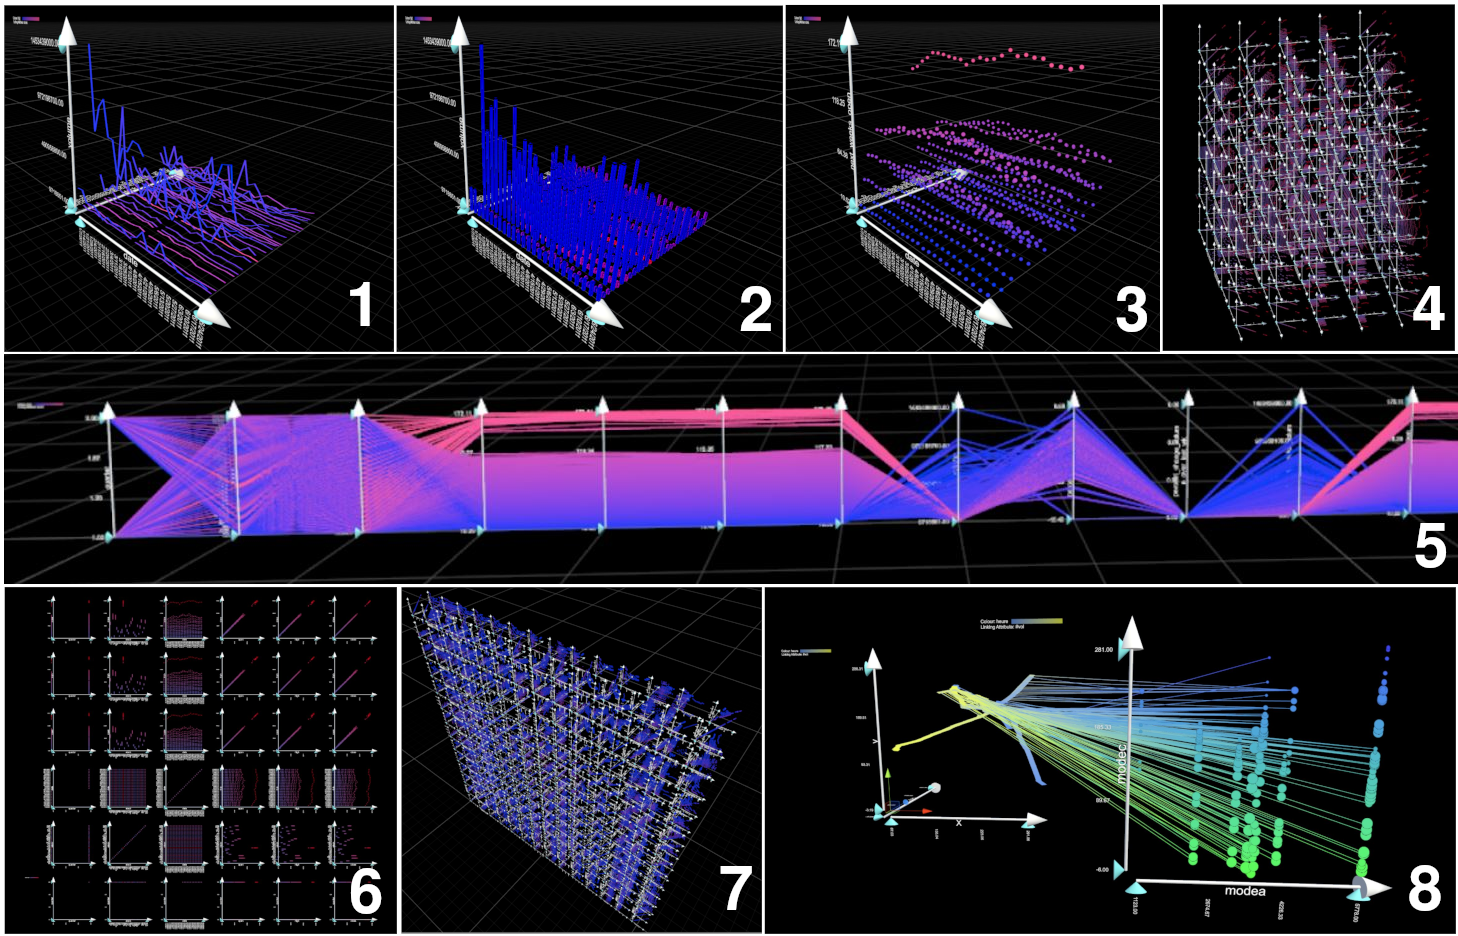
\includegraphics[width=\columnwidth]{iatk}
	\caption[Caption for IATK]{IATK supported visualization types. (1) 3D
		connected dots. (2) 3D bar chart. (3) 3D Scatterplot. (4, 7) 3D
		Scatterplot matrix. (5) Parallel Coordinates Plots. (6) 2D Scatterplot
		matrix. (8) Linked visualizations. The images are from \textsuperscript{1}
		and are in the public domain.}
	\label{fig:iatk_visualizations}
\end{figure}


\smallskip

\noindent IATK integrates an interactive visualization model within its
visualization components that allows a set of interactions including filtering,
brushing and linking (\cref{fig:iatk_visualizations} (8)), details on demand,
animated transitions and attribute-based animations. These interactions are
implemented in the vertex Shader part of the rendering pipeline which leverages
the high parallelism nature of the GPU(s) making them particularly responsive
and efficient at handling large datasets.

\smallskip

\noindent IATK's high-level GUI provides just a small set of built-in visualization
types such as a 3D\textbackslash2D Scatterplot (\cref{fig:iatk_visualizations}
(3)), a parallel coordinates plot (\cref{fig:iatk_visualizations} (5)) or a
3D\textbackslash2D Scatterplot matrix (\cref{fig:iatk_visualizations} (4, 6, 7)).
It also only provides a small set of datapoint geometries. To extend these,
one has to use the provided low-level API which might limit expressiveness for
non-experienced users.

\smallskip

\noindent The authors didn't mention any support for neither real-time data
visualization nor local or remote collaboration. It is also worth mentioning
that for VR, only Scatterplot visualization type is supported. This greatly
limits the expressiveness for VR users.

\subsection{VRIA Toolkit}
Peter et al. introduce VRIA \cite{vria_framework}; a free and open-source \footnote{https://github.com/vriajs}
framework for building IA experiences in VR. Unlike the aforementioned
toolkits, VRIA isn't built as an add-on on top of a game engine. Instead, it is
built upon open-standard Web-based frameworks such as WebVR, A-Frame, React and
D3.js. All of which are mature, open-source and widely used Web-based
frameworks and libraries. This allows VRIA applications to be accessible by a
plethora of VR and non-VR devices.

\smallskip

\noindent The toolkit is designed to be accessible to novices and experts
alike. Similar to DXR, VRIA makes use of a declarative grammar similar to
Vega-Lite \cite{vega_lite} which allows users to create custom visualizations based on a configuration
file. However, this visualization configuration file is only required for
basic functionalities. For extra custom functionalities such as a custom set of
visualization channels, interactions, graphical marks or visualization types,
more experienced users are advised to use the provided low-level API.
VRIA provides The VRIA Builder; a Web application intended for beginners that
integrates a GUI and a 3D scene view to rapidly prototype visualization designs
with instant feedback without having to leave the browser. It is worth
mentioning that, unlike DXR, this customization GUI isn't part of the VR scene
and cannot be viewed withing the VR headset. Only the scene view can be
experienced immersively. However, the authors mentioned their willingness to
add \textit{in-situ} GUI so that users can build and prototype visualizations
iteratively without having to remove the headset and switch back to desktop
screen.

\smallskip

\noindent Thanks to its composable structure, the toolkit can be integrated into
other existing 2D or immersive visualization applications. For instance,
VRIA's visualizations can be overlaid on top of another A-Frame scene.
VRIA has support for collaborative immersive analytics through either the
high-level networking abstraction layer provided by the open-source Networked
A-Frame component or by using the provided API with lower-level networking
libraries.

\smallskip

\noindent In terms of data input, the toolkit only supports tabular data in the form of
JSON or CSV thus real-time data visualization isn't supported. The authors
expressed their willingness to add support for other forms of data models such as
geospatial GeoJSON, network and relational models.

\smallskip

\noindent The authors stated that VRIA offers the option to integrate D3.js
visualization within its IA experiences. D3.js is web-base JavaScript
visualization library that provides a low-level approach to author graphics and
powerful mechanisms to transform and manipulate data. Since D3.js is widely
adopted, integrating it within VRIA allows for easier usability and quicker
authoring of 2D visualizations. However, there wasn't a description of
which D3.js functionalities and visualizations are integrable nor any guidance
on how to integrate it within the VRIA framework.

\smallskip

\noindent More experienced users seeking for a more custom experience are
forced to deal with two separate tools to author custom visualizations;
the visualization configuration file specified in a declarative language and
the API specified in JavaScript. We believe that it would be easier for the end users if VRIA
provided more customizability through the visualization configuration file instead of just
providing very basic functionalities.
Although it is understandable that A-Frame simplifies the process of creating
VR experiences on the web relative to the lower level Three.js library, we
question its necessity. A-Frames' functionalities could be directly implemented
in Three.js thus reducing and simplifying the VRIA stack. The authors stated
their intention to work at the Three.js level directly without the usage of any further
abstraction libraries.

\smallskip

\noindent Whenever 3D graphics are mentioned in the context of web browsers,
performance implementations are one of the most worrying aspects. This is
especially true for Web-based VR applications where two images have to be
rendered each frame preferably at 90 FPS to avoid motion sickness. VRIA's
authors provided visualization benchmarks on a desktop monitor, a desktop
Oculus Rift CV1 and a smartphone. A scatter-plot visualization type was used
with sphere graphical marks. The exact set of visualization channels used
wasn't mentioned neither were attributes of the input data. On the desktop
monitor and Oculus Lift HMD, performance drops significantly after one
thousand data points. On smartphone performance starts dropping at one hundred
data points. This proves that VRIA is not suitable for large dataset
visualizations. The authors claim that the performance observed for the HMD
is similar to that of IATK for the HoloLens device. But the HoloLens uses
its own, much less powerful, hardware while VRIA performance benchmark used
the Oculus Lift CV1 VR HMD which relies on a separate desktop for expensive
rendering operations. We therefore question such comparisons of performance
benchmarks. This is later Web-based XR solutions do not compete,
in terms of performance, with game-engine based solutions.

\smallskip

\noindent VRIA only supports Cartesian plots but the authors expressed their
willingness to add support for other coordinate systems including geographical
and spherical coordinates.
Moreover, although the authors showcased the ease of integrating VRIA with
AR.js to target AR experiences, the absence of an out-of-box support for VRIA
still limits AR accessibility only to experienced users.

\subsection{RagRug Toolkit}

\begin{figure}[tb]
	\centering
	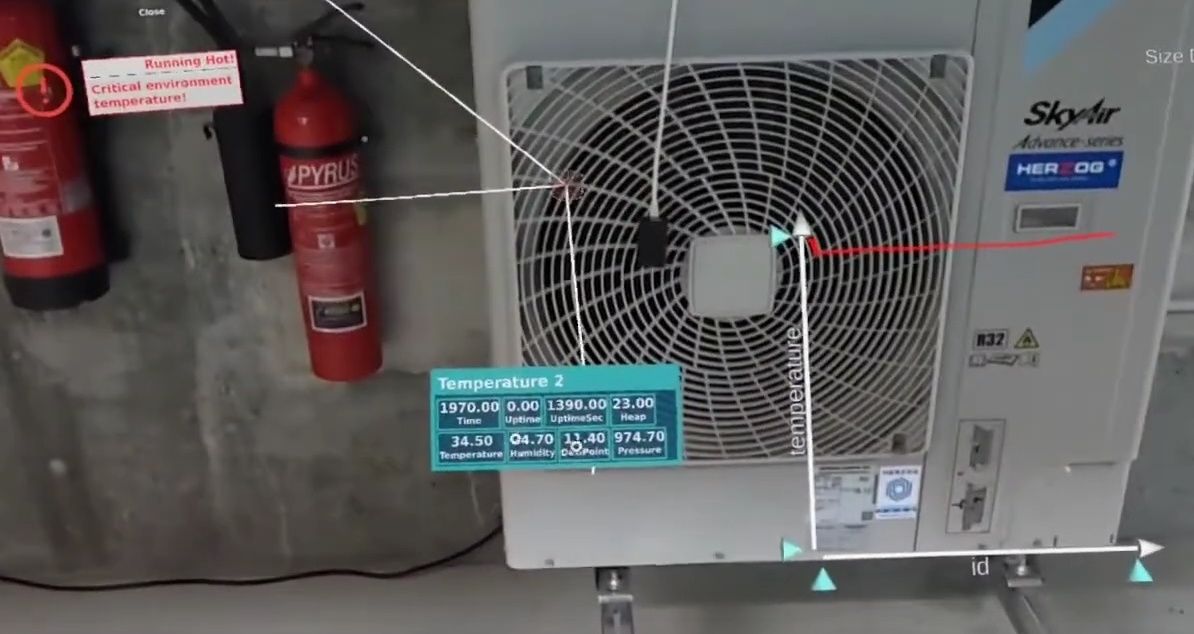
\includegraphics[width=\columnwidth]{ragrug_example}
	\caption[Caption for RagRug]{Example of situated analytics using RagRug
		toolkit. Multiple visualizations are shown and are fed real-time
		temperature data from nearby IOT sensor devices.
		Image from \textsuperscript{4} and is in the public domain. }
	\label{fig:ragrug_example}
\end{figure}

Philipp et al. presented RagRug \cite{ragrug_toolkit}; An open-source
\footnote{https://github.com/philfleck/ragrug} toolkit built on top of IATK
for situated analytics. The term "situated analytics" refers to real-time
data-fed interactive immersive visualizations connected to a meaningful physical
object in close proximity to the user (hereafter we refer to such an object as
a \textit{referent}). For instance, a facility manager equipped with an AR HMD,
when in proximity to an air conditioner with multiple Internet-of-Things (IOT)
sensor devices monitoring temperature and other parameters, multiple real-time
visualizations pop up (\cref{fig:ragrug_example}).

\smallskip

\begin{figure}[tb]
	\centering
	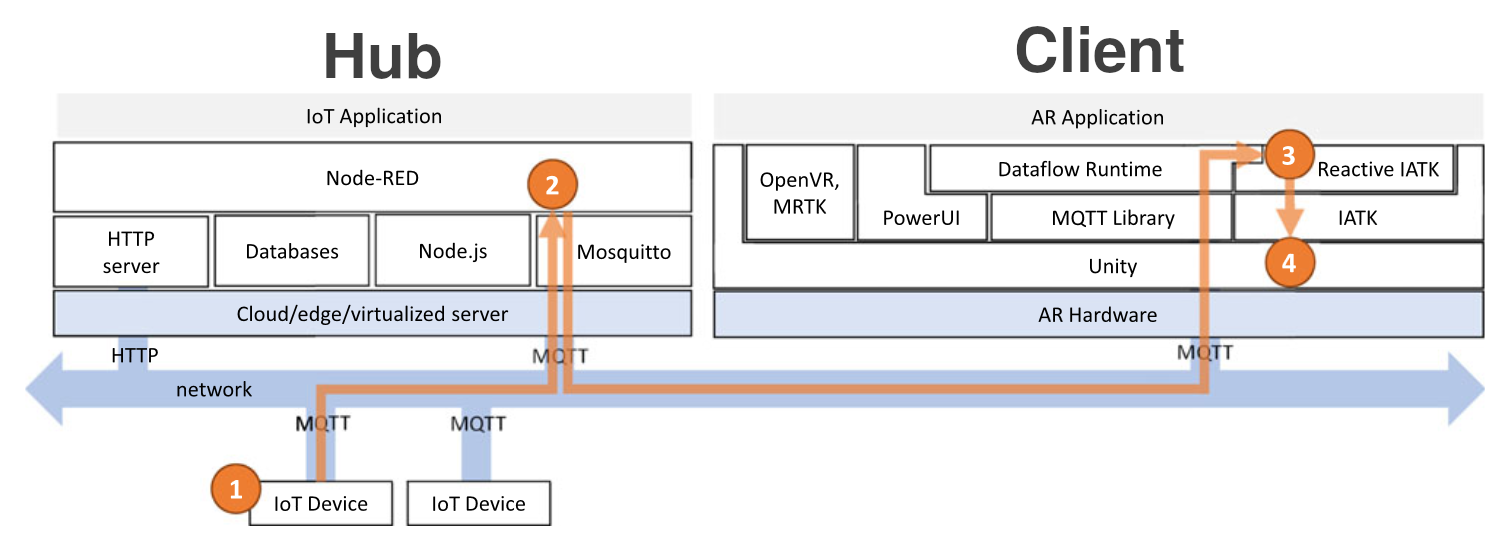
\includegraphics[width=\columnwidth]{ragrug_stack}
	\caption[Caption for RagRug]{RagRug stack. (1) Data is acquired from IoT
		sensors using MQTT. (2) Data filtering. (3) Real-time data is sent to
		IATK as a response to a query. (4) Visualizations are
		rendered/updated in Unity.}
	\label{fig:ragrug_stack}
\end{figure}

\noindent RagRug consists of two standalone platforms, one for experiencing
immersive analytics visualizations and interacting with them (hereafter we
refer to this as the \textit{client}) and one for IoT applications and
databases (hereafter we refer to it as the \textit{hub}). As illustrated
in (\cref{fig:ragrug_stack}) the two platforms make use of the widely adopted
and lightweight MQTT \footnote{https://mqtt.org/} protocol to communicate
data and events.

\smallskip

\noindent The core design goals of RagRug are:
\begin{itemize}
	\item Providing 3D visual encoding: this is already done by IATK
	\item Making visualizations context aware:
	      The tookit should provide visualizations that are context-aware with regards
	      to changes in the real world. For instance, If a referent is moved, the attached
	      visualization should move along with it or if the lighting conditions change
	      then visualization color should adapt to such new conditions or if the user
	      performs an invalid action a notification is adequately shown. RagRug makes
	      use of IoT devices for collecting data about the environment and a cloud server
	      for, among other things, the IoT application logic and depositing data in a
	      database backend so that the client can query it dynamically.
	\item Supporting a comprehensive physical-virtual model: Information about the
	      characteristics of referents such as location, shape or identity should be
	      queried from a suitable database so that the client obtains relevant data
	      dynamically. This is important for correctly linking visualizations to
	      referents.
	\item Making the visualization pipeline reactive: This comes from the IATK's lack
	      of support for neither real-time data (since it expects a static dataset input)
	      nor for receiving events from external sources. To address this, the authors
	      built an extension on top of IATK to update data points on network events
	      locally and externally.
	\item Supporting situated authoring: Since testing situated analytics requires
	      physical interactions with referents, not allowing for situated authoring will
	      result in a cumbersome development experience. To address the lack of in-situ
	      authoring from IATK, The authors make use PowerUI
	      \footnote{https://github.com/Kulestar/powerui}, an open-source JavaScript extension
	      for Unity that allows for UI authoring using CSS, HTML and JavaScript. We find
	      the use of this extension questionable, since it has been deprecated from the
	      Unity Asset store and the open-source GitHub repository has been inactive for
	      more than five years.
\end{itemize}

\smallskip

\noindent The authors provided five application examples with a varied level of
sophistication.

\subsection{Wizualization}

TODO: Is it worth it adding this toolkit (that mainly focuses on interactions)?

\subsection{Comparison}

\section{Prototypes}
\subsection{Uplift}
Barrett et al. proposed Uplift \cite{uplift_prototype}; an in-place
collaborative visual analytics prototype targeting users with diverse
expertise in the domain of microgrids. Uplift is designed for casual visual
analysis use-cases; i.e. to be used to easily identify, in a relatively short
time, key patterns in complex visualized data. The requirements for the
prototype were initially provided and subsequently modified, through multiple
feedback sessions, by a wide range of stakeholders including microgrid project
and energy systems experts.

\smallskip

\begin{figure}[tb]
	\centering
	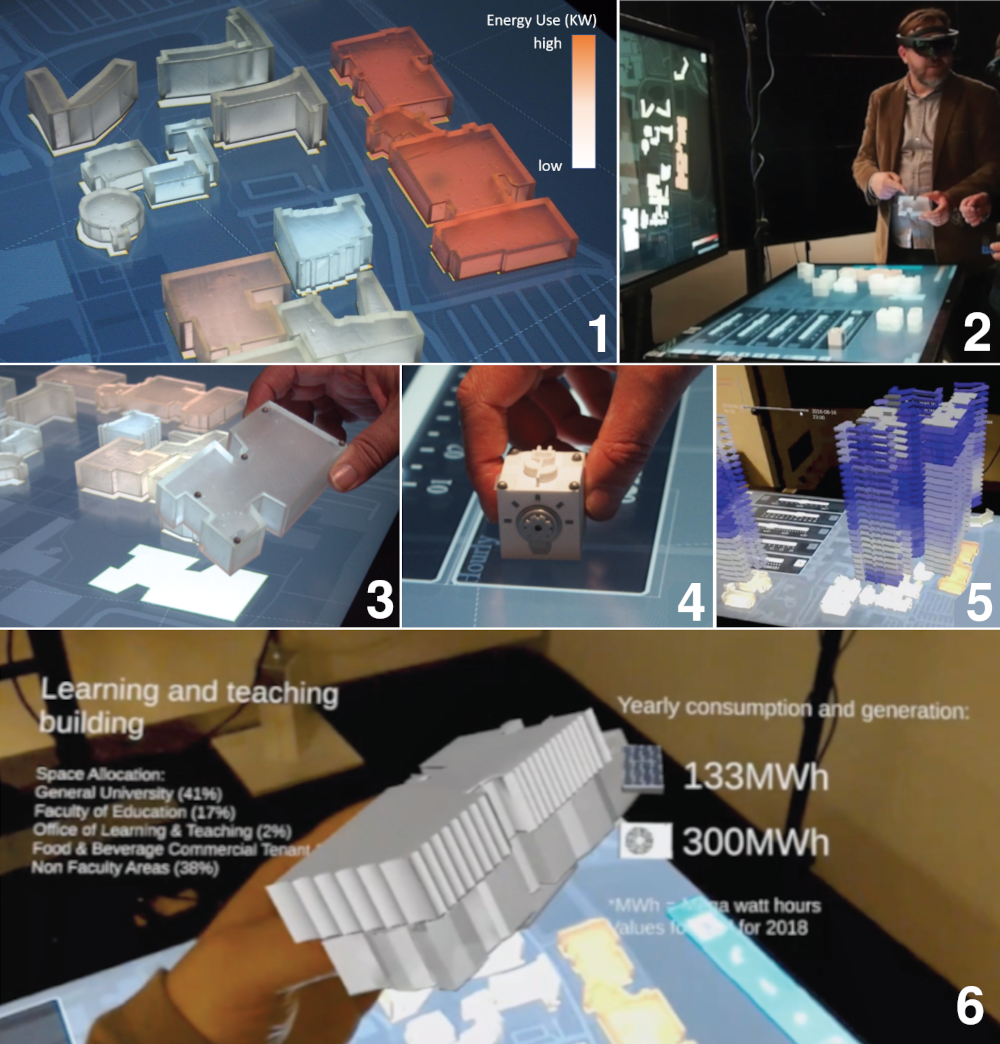
\includegraphics[width=\columnwidth]{uplift}
	\caption[Caption for Uplift]{Uplift. TODO: Add adequate explanations for
		each important Uplift aspect with reference to this figure.}
	\label{fig:uplift}
\end{figure}

\noindent Uplift relies more than just AR headsets to bring casual collaborative visual
analytics to a multitude of microgrid stakeholders. A tabletop display showing
a geographical map of the campus grid is used as a central platform where users
are supposed to gather around and interact with widgets placed on top of it.
Uplift also makes use of tangible
widgets which are physical and interactive elements that control visualization
parameters (for instance by affecting sliders). The prototype also relies on
scaled-down physical models of buildings that are translucent which allows
the color of the surface on which they are placed to be used as an appealing
visualization channel. AR is used to display multiple 3D data types on top of
the tabletop and 2D graphs alongside legends around it. On top of these, Uplift
uses a large display to either replicate the content of the tabletop or show
additional visualizations.

\smallskip

\noindent Through the feedback of 16 participants who tried the prototype, Uplift was
proven to be potentially useful for microgrid-related data analytics.

\smallskip

\noindent Although Uplift was designed for microgrid-related systems,
the authors claim that its applicability domain can be extended to include
other domains that rely on analysis of complex spatial data such as
the construction industry. However, the use of a wide range of technologies
and gadgets makes Uplift a specialized solution that we believe isn't yet
ready for wide deployment. For instance, on top of using Vuforia for tabletop
tracking, Uplift uses an extra proprietary tracking software with four cameras
to track the tangible widgets. Such tracking could have instead been done in
Vuforia therefore removing the need to add cameras to the scene and making the
solution much more self-contained. This is especially true since Vuforia provides
an official plugin for Unity development \cite{unity:vuforia_plugin}.
Moreover, although the topic of real-time monitoring of the microgrid was seen
as beneficial for operators by expert stakeholders, Uplift didn't provide any
solutions to tackle such use case.

\subsection{Conclusion}
TODO: write how these prototypes could be integrated into other toolkits
to enhancing provided IA experiences.

\section{Collaboration Tools and Techniques}
\subsection{Conclusion}
TODO: write how using such tools could contribute to enhancing IA experiences.
\section{Interaction Tools and Techniques}
\subsection{Conclusion}
TODO: write how using such tools could contribute to enhancing IA experiences.
\section{Navigation Tools and Techniques}
\subsection{Conclusion}
TODO: write how using such tools could contribute to enhancing IA experiences.
\section{Transition and Animation Tools and Techniques}
TODO: add introduction with suitable references for importance of animations
and cross-virtuality transitions.
\subsection{HybridAxes Tool}
Mohammad et al. introduced HybridAxes \cite{hybridaxes_tool}; an extension of
IATK toolkit that allows for a smooth interoperability between 2D desktop
visualizations and immersive reality experiences (\cref{fig:hybridaxes}).

\medskip

\begin{figure}[tb]
	\centering
	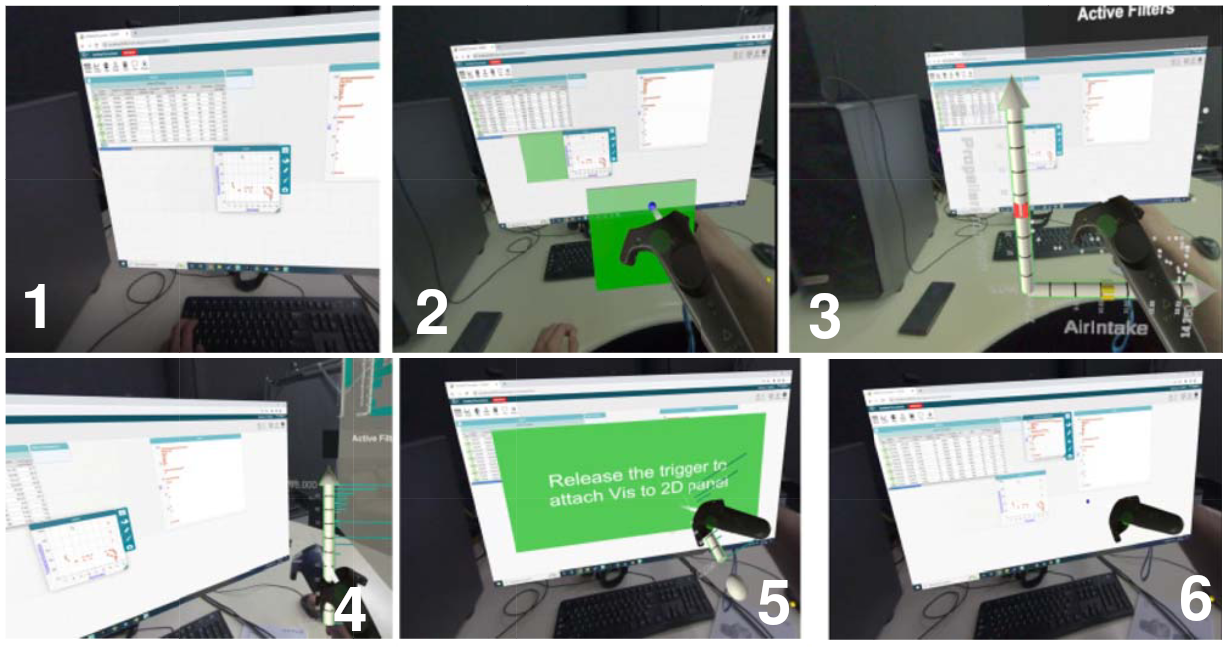
\includegraphics[width=\columnwidth]{hybridaxes}
	\caption[Caption for RagRug]{HybredAxes context switch processes. (1, 2, 3)
		Pulling data/visualization from a 2D screen. (4, 5, 6) Pushing a
		visualization to a 2D screen from an immersive AR environment.}
	\label{fig:hybridaxes}
\end{figure}

\noindent HybridAxes aims to provide a balanced feature set and performance
between the two ends of the Reality-Virtuality continuum while giving the users the ultimate choice to choose
which environment to work in. To avoid disruptions of the user's
flow when context switching, the tool also aims to provide a smooth transition
by reducing visualization generation delays. It claims to do that by
anticipating the user's interactions in both modes and preemptively generating
visualizations in the background. Moreover, the authors stated that providing
a clear signaling of transition status either through visual (\cref{fig:hybridaxes} (2, 5)) or
controller-related feedback is a core design requirement for the tool.
Keeping the same values for the visualization channels, if possible, when
transitioning a visualization between the two experiences is also stated as
a core design goal. HybridAxes should also provide support for synchronized
cross-virtuality brushing and linking. For instance, a user may have a tabular
data on a 2D desktop alongside a 3D scatterplot in the immersive environment.
When highlighting an entry in the table, associated datapoints in the
scatterplot should also be highlighted. HybridAxes, aims to also favor desktop
for interactions that require the detailed manipulation of text entries. The
choice of interaction method, either through free-hand or
controller-based interactions, is given to the user.

\medskip

\noindent In terms of implementation, HybridAxes adopts CODAP; an open-source
\footnote{https://codap.concord.org} visual analytics tool, alongside a plugin
that enables the desktop system to receive commands via a Websocket interface.
A Node.js-based Websocket server is used to relay the messages between Unity
and the desktop system. We question the use of these extra tools and frameworks
since we believe that transitioning between immersive and 2D Unity
visualizations is superior to the suggested workflow. Our main argument is
that this way all visualizations are established within one framework - Unity -
which therefore allows for a more versatile, accessible and easier-to-use
toolkit. The tool provides support for the same set of visualizations as IATK
maninly: scatterplots, parrallel coordinate plots and bar charts.

\medskip

\noindent In terms of performance, the authors claim that anticipating user
actions has resulted in smoother experience. However, no comparative
performance measurements were provided to back this claim.

\smallskip

\noindent In terms of interactions, three types are supported:
\begin{itemize}
	\item Pull visualizations from the 2D desktop by using free-hand gestures
	      or the controller(s) (\cref{fig:hybridaxes} (1, 2, 3)).
	\item Push visualizations from the immersive environment back to the 2D
	      desktop (\cref{fig:hybridaxes} (4, 5, 6)).
	\item Brush datapoints on either side of the environments and see their
	      counterparts in the other side get highlighted.
\end{itemize}


\noindent The authors hypothesize that enabling visual analytics users to
smoothly context switch between a 2D screen and 3D immersive experience could
improve their sense-making abilities. A limited study of the usefulness of the tool has been conducted on just four
participants where they analyzed the data in three scenarios: 1) just using 2D
desktop screen, 2) using a hybrid desktop/AR system and 3) just using the AR
system. The authors claim that the study results align with their hypothesis.
However, neither metrics nor sufficient details were provided to prove this
claim. Nonetheless, the authors mentioned their willingness to perform a more
rigorous study in the future.

\subsection{Conclusion}
TODO: write how using such tools could contribute to enhancing IA experiences.

\section{Conclusion}
TO BE WRITTEN AT THE VERY END

\acknowledgments{TO BE WRITTEN AT THE VERY END}
\printbibliography
\end{document}
